% !TeX root = ../main.tex
% Add the above to each chapter to make compiling the PDF easier in some editors.

\chapter{Derivative Works of 3DGS}\label{chapter:derivative_models}

% Mainly: Describe the main methodology, the key features, differences to the original model, compare
In this chapter, we briefly go through each Gaussian Splatting model used in this research.

\section{2D Gaussian Splatting}

Two-dimensional Gaussian Splatting (2DGS) \parencite{2DGS} is a derivative work based on the original 3DGS technique. One of the main goals of 2DGS is to be able to create a multi-view-accurate surface representation of a scene, which is a main weakness of its predecessor \parencite{3DGS}. 3DGS, while able to achieve high-quality results in real time, is unable to represent surfaces of objects in the scene accurately due to its lack of explicit surface representation. 3D Gaussians are optimized independently without looking at the overall structure of the scene, which leads to it not being coherent with each other. This means that when we try to look at the overall result from different perspective, the overall geometry of the scene may appear to change. The main difference of 2DGS is that instead of using 3D Gaussians, it focuses on using 2D Gaussians, which allows for more accurate surface reconstruction and view-consistent geometry reconstruction using intrinsic modelling of surfaces. Processed values are then regularized through depth distortion and normal consistency. Through these means, 2DGS is able to create more geometrically-accurate surfaces while maintaining fast training and rendering speed.

\subsection{Modeling and Splatting of Gaussians}

As aforementioned, 2DGS employs the usage of 2D Gaussians instead of 3D Gaussians in an effort to provide better alignment with thin surfaces. 2D Gaussians are planar elliptical disc-like two-dimensional structures which possess a center point \(p_k\), two tangential vectors \(t_u\) and \(t_v\), and two scaling factors \(s_u\) and \(s_v\), combined into a scaling vector \(S = (s_u, s_v)\) to control the variance. The variance of a Gaussian describes how elliptical or circular a Gaussian is in each axes, while the tangential vectors describe the orientation and can be arranged into a \(3 \times 3\) rotation matrix \(\mathbf{R}=[t_u, t_v, t_w]\) with \(t_w = t_u \times t_v\). The scaling factor can also be converted into a \(3 \times 3\) diagonal matrix \(\mathbf{S}\) with zero as its last entry.

In a local tangent plane, a 2D Gaussian is described as follows:

\begin{center}
    \(P(u, v) = p_k + s_u t_u u + s_v t_v v = \mathbf{H}(u, v, 1, 1)^T\)

    where \(\mathbf{H}=
    \begin{bmatrix}
        s_u t_u & s_v t_v & 0 & p_k \\
        0       & 0       & 0 & 1
    \end{bmatrix} 
    =
    \begin{bmatrix}
        \mathbf{R}S & p_k \\
        0           & 1
    \end{bmatrix}\)
\end{center}

In order to evaluate the value of a certain 2D Gaussian at a certain point \(\mathbf{u} = (u, v)\) we can use the following formula:

\begin{center}
    \(\mathcal{G}(u) = exp(-\frac{u^2 + v^2}{2})\)
\end{center}

In 2DGS, center point \(p_k\), scaling \(S = (s_u, s_v)\), as well as rotation \((t_u, t_v)\) are learnable parameters. Additional parameters opacity \(\alpha\) and view-dependent appearance \(c\) are also attached to each Gaussians.

For the splatting process, a formula based on homogeneous coordinates \parencite{splatting} is used:

\begin{center}
    \(\mathbf{x} = (xz, yz, z, z)^T = \mathbf{W}P(u,v) = \mathbf{WH}(u, v, 1, 1) ^ T\),
\end{center}

where \(\mathbf{x}\) represents 2D coordinates \((x, y)\) in screen space point and \(z\) represents depth at ray-splat intersection.

For the rasterization process, explicit ray-splat intersection \parencite{rayintersect} method is used in order to avoid ill-conditioned transformations induced by the usage of implicit methods \parencite{splatting}. Given a coordinate point \(\mathbf{x} = (x, y)\), a ray being shot into the scene is parametrized as the intersection of the \(x\)-plane and the \(y\)-plane, where the \(x\)-plane can be represented as \(\mathbf{h}_x = (-1, 0, 0, x)^T\) and the \(y\)-plane can similarly be represented as \(\mathbf{h}_y = (0, -1, 0, y)^T\). Afterwards, a transformation matrix \(\mathbf{M} = (\mathbf{WH})^{-1} = (\mathbf{WH})^T\) is used to transform both planes into the local coordinate system of the 2D Gaussian primitives, yielding:

\begin{center}
    \(h_u = (\mathbf{WH})^Th_x\) and \(h_v = (\mathbf{WH})^Th_y\),
    with \(h_u \cdot (u, v, 1, 1)^T = h_v \cdot (u, v, 1, 1)^T = 0\)
\end{center}

For the intersection point \(\mathbf{u}(x)\), the solution is:
\begin{center}
    \(u(x) = \frac{h^2_uh^4_v - h^4_uh^2_v}{h^1_uh^2_v - h^2_uh^1_v}\) and
    \(v(x) = \frac{h^4_uh^1_v - h^1_uh^4_v}{h^1_uh^2_v - h^2_uh^1_v}\), 
    
    with \(h^i_u and h^i_v\) as \(i\)-th parameter of the 4D plane and 
    \(h^3_u and h^3_v = 0\)
\end{center}

Due to the usage of 2D Gaussians, when observed from specific standpoints the shape will degenerate into a line and could then be missed in the rasterization process. To overcome this, object-space low-pass filter is used \parencite{lowpass}:

\begin{center}
    \(\hat{\mathcal{G}}(x) = max\{\mathcal{G}(\mathbf{u}(x)), \mathcal{G}(\frac{x - c}{\sigma})\}\),
    with \(c\) as the projection of center point \(p_k\).
\end{center}

This low-pass filter essentially "fixes" the minimum value of the Gaussians so that such small-valued Gaussians are not be missed during the rendering process. This value is, in this case, bounded by a filter with center \(c\) and radius \(\sigma\) with a fixed value of \(\sigma = \frac{\sqrt{2}}{2}\). 

Next, for the actual rasterization, a process similar to 3DGS is used. First, bounding boxes are computed for each Gaussians and then these Gaussians are sorted and organized based on the depth of its center point into their respective bounding boxes. As in 3DGS, alpha front-to-back blending is then used during rendering:

\begin{center}
    \(\mathbf{c(x)} = \sum\limits_{i = 1} (\mathbf{c}_i \alpha_i \hat{\mathcal{G}}_i (\mathbf{u(x)})\prod\limits_{j = 1}^{i - 1} (1 - \alpha_j \hat{\mathcal{G}}_j(\mathbf{u(x)}))\)
\end{center}

\subsection{Training of 2DGS Models}

During the training process, two regularization terms: 1) depth distortion and 2) normal consistency are introduced. This is done in an effort to prevent too much noise during reconstruction. Depth distortion is first introduced by the predecessor of 2DGS, Mip-NeRF360 \parencite{mipnerf} to prevent "background collapse" phenomenon, in which distant surfaces are incorrectly modeled as semi-transparent. In 2DGS, depth distortion is done to minimize distance between ray-splat intersections and encourage concentration of weight distribution along the rays:

\begin{center}
    \(\mathcal{L}_d = \sum\limits_{i, j} w_iw_j|z_i - z_j|\),
\end{center}
with \(\omega_i = \alpha_i \hat{\mathcal{G}}_i(\mathbf{u(x)}) \prod\limits_{j = 1}^{i - 1} (1 - \alpha_j \hat{\mathcal{G}}_j(\mathbf{u(x)}))\) as blending weight of the \(i\)-th intersection and \(z_i\) as depth of its intersection points.

The second term, normal consistency, is used to guarantee that the 2D Gaussians are locally aligned with surfaces having an accumulated opacity of 0.5 at median intersection point \(p_s\), such that the 2D Gaussians are able to be an approximate to the actual object's surface:

\begin{center}
    \(\mathcal{L}_n = \sum\limits_i \omega_i(1 - n_i^TN)\),
\end{center}
with \(i\) as index indicator of the number of intersecting splats along the ray, \(\omega\) as blending weight of the intersection points, \(n_i\) as normal of the \(i\)-th splat, oriented towards the camera position, and \(N\) as normal estimated by the gradient of the depth map:

\begin{center}
    \(N(x, y) = \frac{\nabla_x p_s \times \nabla_y p_s}{|\nabla_x p_s \times \nabla_y p_s|}\)
\end{center}

\subsection{Limitations of 2DGS}

Although 2DGS is able to achieve accurate geometric modeling of 3D scenes, it suffers from some limitations still. In 2DGS, surfaces are assumed to always be at full opacity, which means that there will be problems when dealing with glass and other semi-transparent surfaces. Another limitation of 2DGS is that through its usage of depth distortion regularization and oversmoothing, the reconstruction tends to be less accurate on structures with fine details. There is a trade-off between image quality and geometry happening here; fixed, smooth structures are more preferred and due to this, the reconstruction process will view extra details as mere noise and smooth it over.

\section{RaDe-GS}

Rasterizing Depth in Gaussian Splatting (RaDe-GS) \parencite{radegs} is a further attempt to improve geometric reconstruction in Gaussian Splatting while addressing problems faced by 2DGS with quality reductions and rendering efficiency. This is done by creating a rasterized approach to render depth maps and surface normal maps of 3D Gaussians. Through this strategy, RaDe-GS is able to improve the reconstruction accuracy and computational efficiency and even achieve a Chamfer distance error comparable to NeuraLangelo \parencite{neuralangelo}, a Neural Surface Reconstruction method spearheaded by projects such as NeuS \parencite{neus} and UNISURF \parencite{unisurf}, on the DTU dataset.

\subsection{Splatting Method}

RaDe-GS closely follows basic 3DGS method \parencite{3DGS} for scene representation using 3D Gaussians. The usage and definition of 3D Gaussians stays the same in both works, and RaDe-GS also employs approximations for perspective camera projections and the usage of alpha blending to determine color (see 3DGS explanation for complete equation on 3D Gaussians, approximation of local affine projections, and alpha blending).     

\subsection{Rasterizing Depth for Splats}

Unlike its predecessors, RaDe-GS adopts a rasterized approach for the efficient evaluation of the depth of each Gaussians. This is done in order to preserve the finer details of the objects being reconstructed. With this method, the depth calculation of a projected 2D Gaussian is as follows:

\begin{center}
    \(d = z_c + p 
    \begin{bmatrix}
        \Delta u \\
        \Delta v
    \end{bmatrix}
    \),
\end{center}
where \((u_c, v_c)\) is the center point of the Gaussian, \(z_c\) is the depth of the center point of the Gaussian, \(\Delta u = u_c - u\) and \(\Delta v = v_c - v\) are relative positions of the pixel in coordinate point \((u, v)\), and \(p \in \mathbb{R}^2\) is a \(1 \times 2\) vector determined by Gaussian parameters and camera extrinsic parameters.

Surface normal directions as projected by the Gaussians are then calculated by taking intersecting points and forming a plane in ray space with these points (indicated by the green line in Figure \ref{fig:radegs-ray-space}).

\begin{figure}[h]
    \centering
    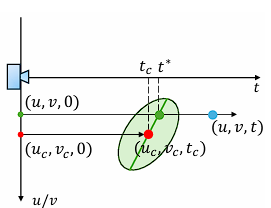
\includegraphics[width=0.5\linewidth]{figures/radegs-ray-space.png}
    \caption{Plane formed in ray space by intersecting points. \parencite{radegs}}
    \label{fig:radegs-ray-space}
\end{figure}

The normal direction of the projected Gaussian can then be regarded as the plane's normal direction and then transformed into camera space for normal map computation.

\subsection{Limitations of RaDe-GS}

Although able to reproduce highly-sophisticated depth information during the reconstruction process and providing a solid improvement to the general 3DGS method, there are some questions that arose from the usage of RaDe-GS in more realistic scenarios. First, even though RaDe-GS is able to provide more sophisticated geometrical details when compared to previous methods like 2DGS that suffers from oversmoothing, it may still be unable to perform well in scenes with a lot of noise, since it does not employ any particular strategies to filter out noise. Moreover, it still does not address the problem with special types of reflective surface that 2DGS also suffers from.

\section{GS2Mesh}

GS2Mesh \parencite{gs2mesh} is another novel approach aimed to address the issue of accurate geometric representation in Gaussian Splatting methods. Unlike the traditional Gaussian Splatting method \parencite{3DGS} where geometry is immediately extracted out of the properties of the created Gaussians, GS2Mesh aims to do this by extracting geometry through a pre-trained stereo-matching model instead. Stereo-aligned pairs of images corresponding to the original poses are rendered and fed into a stereo model to get depth information and then fused together to form a single mesh. This results in a much smoother and more accurate reconstruction that still maintains intricate details when compared to 2DGS \parencite{2DGS}.

\subsection{GS2Mesh Pipeline}

GS2Mesh accepts videos or a collection of images of a static scene as input. This input is then passed on to COLMAP \parencite{colmap1} \parencite{colmap2}, a general-use Structure-from-Motion (SfM) pipeline that is used to deduce camera matrices and identify corresponding image pairs and also points of interests from the corresponding input images.

Afterwards, the output from COLMAP is then passed on to the 3DGS model \parencite{3DGS}, where 3D Gaussians are identified and optimized based on photometric loss of the input images when compared to the corresponding rendered images. A scene reconstruction is then created in this process. GS2Mesh pipeline then generates novel stereo views of the scene to form an image pair of the same pose \((R_L, T_L)\) to be paired together. The left image is first generated directly from the training images, and the right images are then created by shifting it along a horizontal baseline \(b\) in such a way that the pair is stereo-calibrated:

\begin{center}
    \(R_R = R_L, T_R = T_L + (R_L \times [b, 0, 0])\),
\end{center}
with \(R\) as the rotation matrix of the pose and T the translation vector.

Next, the stereo-calibrated image pairs are inputted into a stereo matching algorithm with the objective of forming depth profiles for every image pairs. Here, the DLNR model \parencite{dlnr} is used, as it can be considered as the state-of-art neural stereo matching model at the time. During this process, an occlusion mask is first applied to mask parts of the scene that is only visible from one side of the cameras. Consequently, a second mask that filters out objects that are too close to the camera is applied. This is done since current stereo matching algorithms are inaccurate when dealing with such objects; the stereo matching error itself can be described as such:

\begin{center}
    \(\epsilon(Z) \approx \frac{\epsilon(d)}{f_x \cdot B} Z^2\) \parencite{stereo-error},
\end{center}
with \(\epsilon(d)\) as disparity output error, \(Z\) as ground truth depth, \(\epsilon(Z)\) as error of depth estimate, \(f_x\) as the camera's horizontal focal length, and \(B\) as baseline, which with further experiments is then fixed at 7\% of the scene radius. Thus, simply eliminating the objects with the hopes that it will be covered by a more appropriate image pair is reasonable to improve the accuracy of the model. Finally, a Truncated Signed Distance Function (TSDF) algorithm \parencite{tsdf} is applied, followed by the Marching-Cubes meshing algorithm \parencite{marchingcubes} in order to generate a polygonal mesh as output.

\subsection{Limitations of GS2Mesh}

Since GS2Mesh mainly focuses on creating a pipeline that would maximize the traditional 3DGS method, it still retains some of the weaknesses of 3DGS. One weakness is that it tends to produce noisy results, especially in areas that are not sufficiently covered by the input images. It also still has not addressed the main limitation of more recent models like 2DGS and RaDe-GS: transparent surfaces. Furthermore, the usage of TSDF fusion process is not efficient for larger inputs; rendering these take up a large amount of resources and is extremely inefficient.


